\documentclass{beamer}
% Setup for bibliography
\usepackage[
backend=biber,
style=numeric-comp,
]{biblatex}
\addbibresource{../../references.bib}

% Pretty self explanatory
% We sue this in title bits
\usepackage{datetime}

% Standard math packages / setup
\usepackage{amsmath} 
\usepackage{amsfonts}
\usepackage{amsthm}
\usepackage{amssymb} 
\usepackage{accents}
\usepackage{mathrsfs}
\usepackage{mathtools}

\usepackage{bm}

%\newtheorem{lemma}{Lemma}
%\newtheorem{theorem}{Theorem}
%\newtheorem{definition}{Definition}

% So we can import pngs
\usepackage{graphicx} 

% This gives us nice clickable links 
% https://www.overleaf.com/learn/latex/Hyperlinks#Styles_and_colours
\usepackage{hyperref}
\hypersetup{
    colorlinks=true,
    linkcolor=blue,
    citecolor=blue,
    filecolor=magenta,      
    urlcolor=cyan,
    pdftitle={Monte Carlo Methods (DRAFT)},
    pdfpagemode=FullScreen,
    }
\urlstyle{same}

% Allows us to define colors
% We use this in the next block, listings
\usepackage{color}
\definecolor{dkgreen}{rgb}{0,0.6,0}
\definecolor{gray}{rgb}{0.5,0.5,0.5}
\definecolor{mauve}{rgb}{0.58,0,0.82}

% Allows us to include 
\usepackage{listings}
\lstset{frame=tb,
  language={},
  aboveskip=3mm,
  belowskip=3mm,
  showstringspaces=false,
  columns=flexible,
  basicstyle={\small\ttfamily},
  numbers=none,
  numberstyle=\tiny\color{gray},
  keywordstyle=\color{blue},
  commentstyle=\color{dkgreen},
  stringstyle=\color{mauve},
  breaklines=true,
  breakatwhitespace=true,
  tabsize=4
}

% Adds bulletized outlines with outline environment
\usepackage{outlines}

% Tikz
\usepackage{tikz}

% Colors
\usepackage{xcolor}
\definecolor{uconnblue}{rgb}{0.08, 0.18, 0.28}
\definecolor{intactblue}{rgb}{0.13, 0.26, 0.45}
\definecolor{mastercamred}{rgb}{0.83, 0.01, 0.23}

% By default beamer slides are 4:3 , 128mm by 96mm

\logo{
\includegraphics[height=0.5cm]{../../assets/SBU_logos/horz_2clr_rgb_300ppi.png}}

\usetheme{CambridgeUS}

\AtBeginSection[]
{
  \begin{frame}
    \frametitle{Table of Contents}
    \tableofcontents[currentsection]
  \end{frame}
}

% \shadowimage[width=8cm]{image}
%
% Provides a drop-shadow to images
%
% From
% https://tex.stackexchange.com/questions/81842/creating-a-drop-shadow-with-guassian-blur 
\usetikzlibrary{shadows,calc}

% code adapted from https://tex.stackexchange.com/a/11483/3954

% some parameters for customization
\def\shadowshift{3pt,-3pt}
\def\shadowradius{6pt}

\colorlet{innercolor}{black!60}
\colorlet{outercolor}{gray!05}

% this draws a shadow under a rectangle node
\newcommand\drawshadow[1]{
    \begin{pgfonlayer}{shadow}
        \shade[outercolor,inner color=innercolor,outer color=outercolor] ($(#1.south west)+(\shadowshift)+(\shadowradius/2,\shadowradius/2)$) circle (\shadowradius);
        \shade[outercolor,inner color=innercolor,outer color=outercolor] ($(#1.north west)+(\shadowshift)+(\shadowradius/2,-\shadowradius/2)$) circle (\shadowradius);
        \shade[outercolor,inner color=innercolor,outer color=outercolor] ($(#1.south east)+(\shadowshift)+(-\shadowradius/2,\shadowradius/2)$) circle (\shadowradius);
        \shade[outercolor,inner color=innercolor,outer color=outercolor] ($(#1.north east)+(\shadowshift)+(-\shadowradius/2,-\shadowradius/2)$) circle (\shadowradius);
        \shade[top color=innercolor,bottom color=outercolor] ($(#1.south west)+(\shadowshift)+(\shadowradius/2,-\shadowradius/2)$) rectangle ($(#1.south east)+(\shadowshift)+(-\shadowradius/2,\shadowradius/2)$);
        \shade[left color=innercolor,right color=outercolor] ($(#1.south east)+(\shadowshift)+(-\shadowradius/2,\shadowradius/2)$) rectangle ($(#1.north east)+(\shadowshift)+(\shadowradius/2,-\shadowradius/2)$);
        \shade[bottom color=innercolor,top color=outercolor] ($(#1.north west)+(\shadowshift)+(\shadowradius/2,-\shadowradius/2)$) rectangle ($(#1.north east)+(\shadowshift)+(-\shadowradius/2,\shadowradius/2)$);
        \shade[outercolor,right color=innercolor,left color=outercolor] ($(#1.south west)+(\shadowshift)+(-\shadowradius/2,\shadowradius/2)$) rectangle ($(#1.north west)+(\shadowshift)+(\shadowradius/2,-\shadowradius/2)$);
        \filldraw ($(#1.south west)+(\shadowshift)+(\shadowradius/2,\shadowradius/2)$) rectangle ($(#1.north east)+(\shadowshift)-(\shadowradius/2,\shadowradius/2)$);
    \end{pgfonlayer}
}

% create a shadow layer, so that we don't need to worry about overdrawing other things
\pgfdeclarelayer{shadow} 
\pgfsetlayers{shadow,main}


\newcommand\shadowimage[2][]{%
\begin{tikzpicture}
\node[anchor=south west,inner sep=0] (image) at (0,0) {\includegraphics[#1]{#2}};
\drawshadow{image}
\end{tikzpicture}}



%Information to be included in the title page:
\title{Taichi: An Introduction}
\author{Russell Bentley}
\institute{Stony Brook}
\date{2024}

\begin{document}

\frame{\titlepage}

\begin{frame}{Taichi?}
\begin{columns}
\column{0.48\linewidth}
\centering
\begin{outline}
  \1 Parallelized Compute Kernel Compiler
    \2 Focused on graphics use-cases 
  \1 Based on Yuanming Hu's (?) Thesis
    \2 Conference Paper for ACM  
\end{outline}
\column{0.48\linewidth}
\centering
\shadowimage[width=2.5cm]{yuanming_hu.png} 

\shadowimage[width=2.5cm]{taichi_paper.png} 

\end{columns}
\end{frame}

\begin{frame}{Useful Links}
\begin{columns}
\column{0.48\linewidth}
\centering
\begin{outline}
  \1 Taichi homepage: \url{https://www.taichi-lang.org}
  \1 Official docs / guides: \url{https://docs.taichi-lang.org}
  \1 API reference: \url{https://docs.taichi-lang.org/api/}
  \1 Github: \url{https://github.com/taichi-dev/taichi}
\end{outline}
\column{0.48\linewidth}
\centering
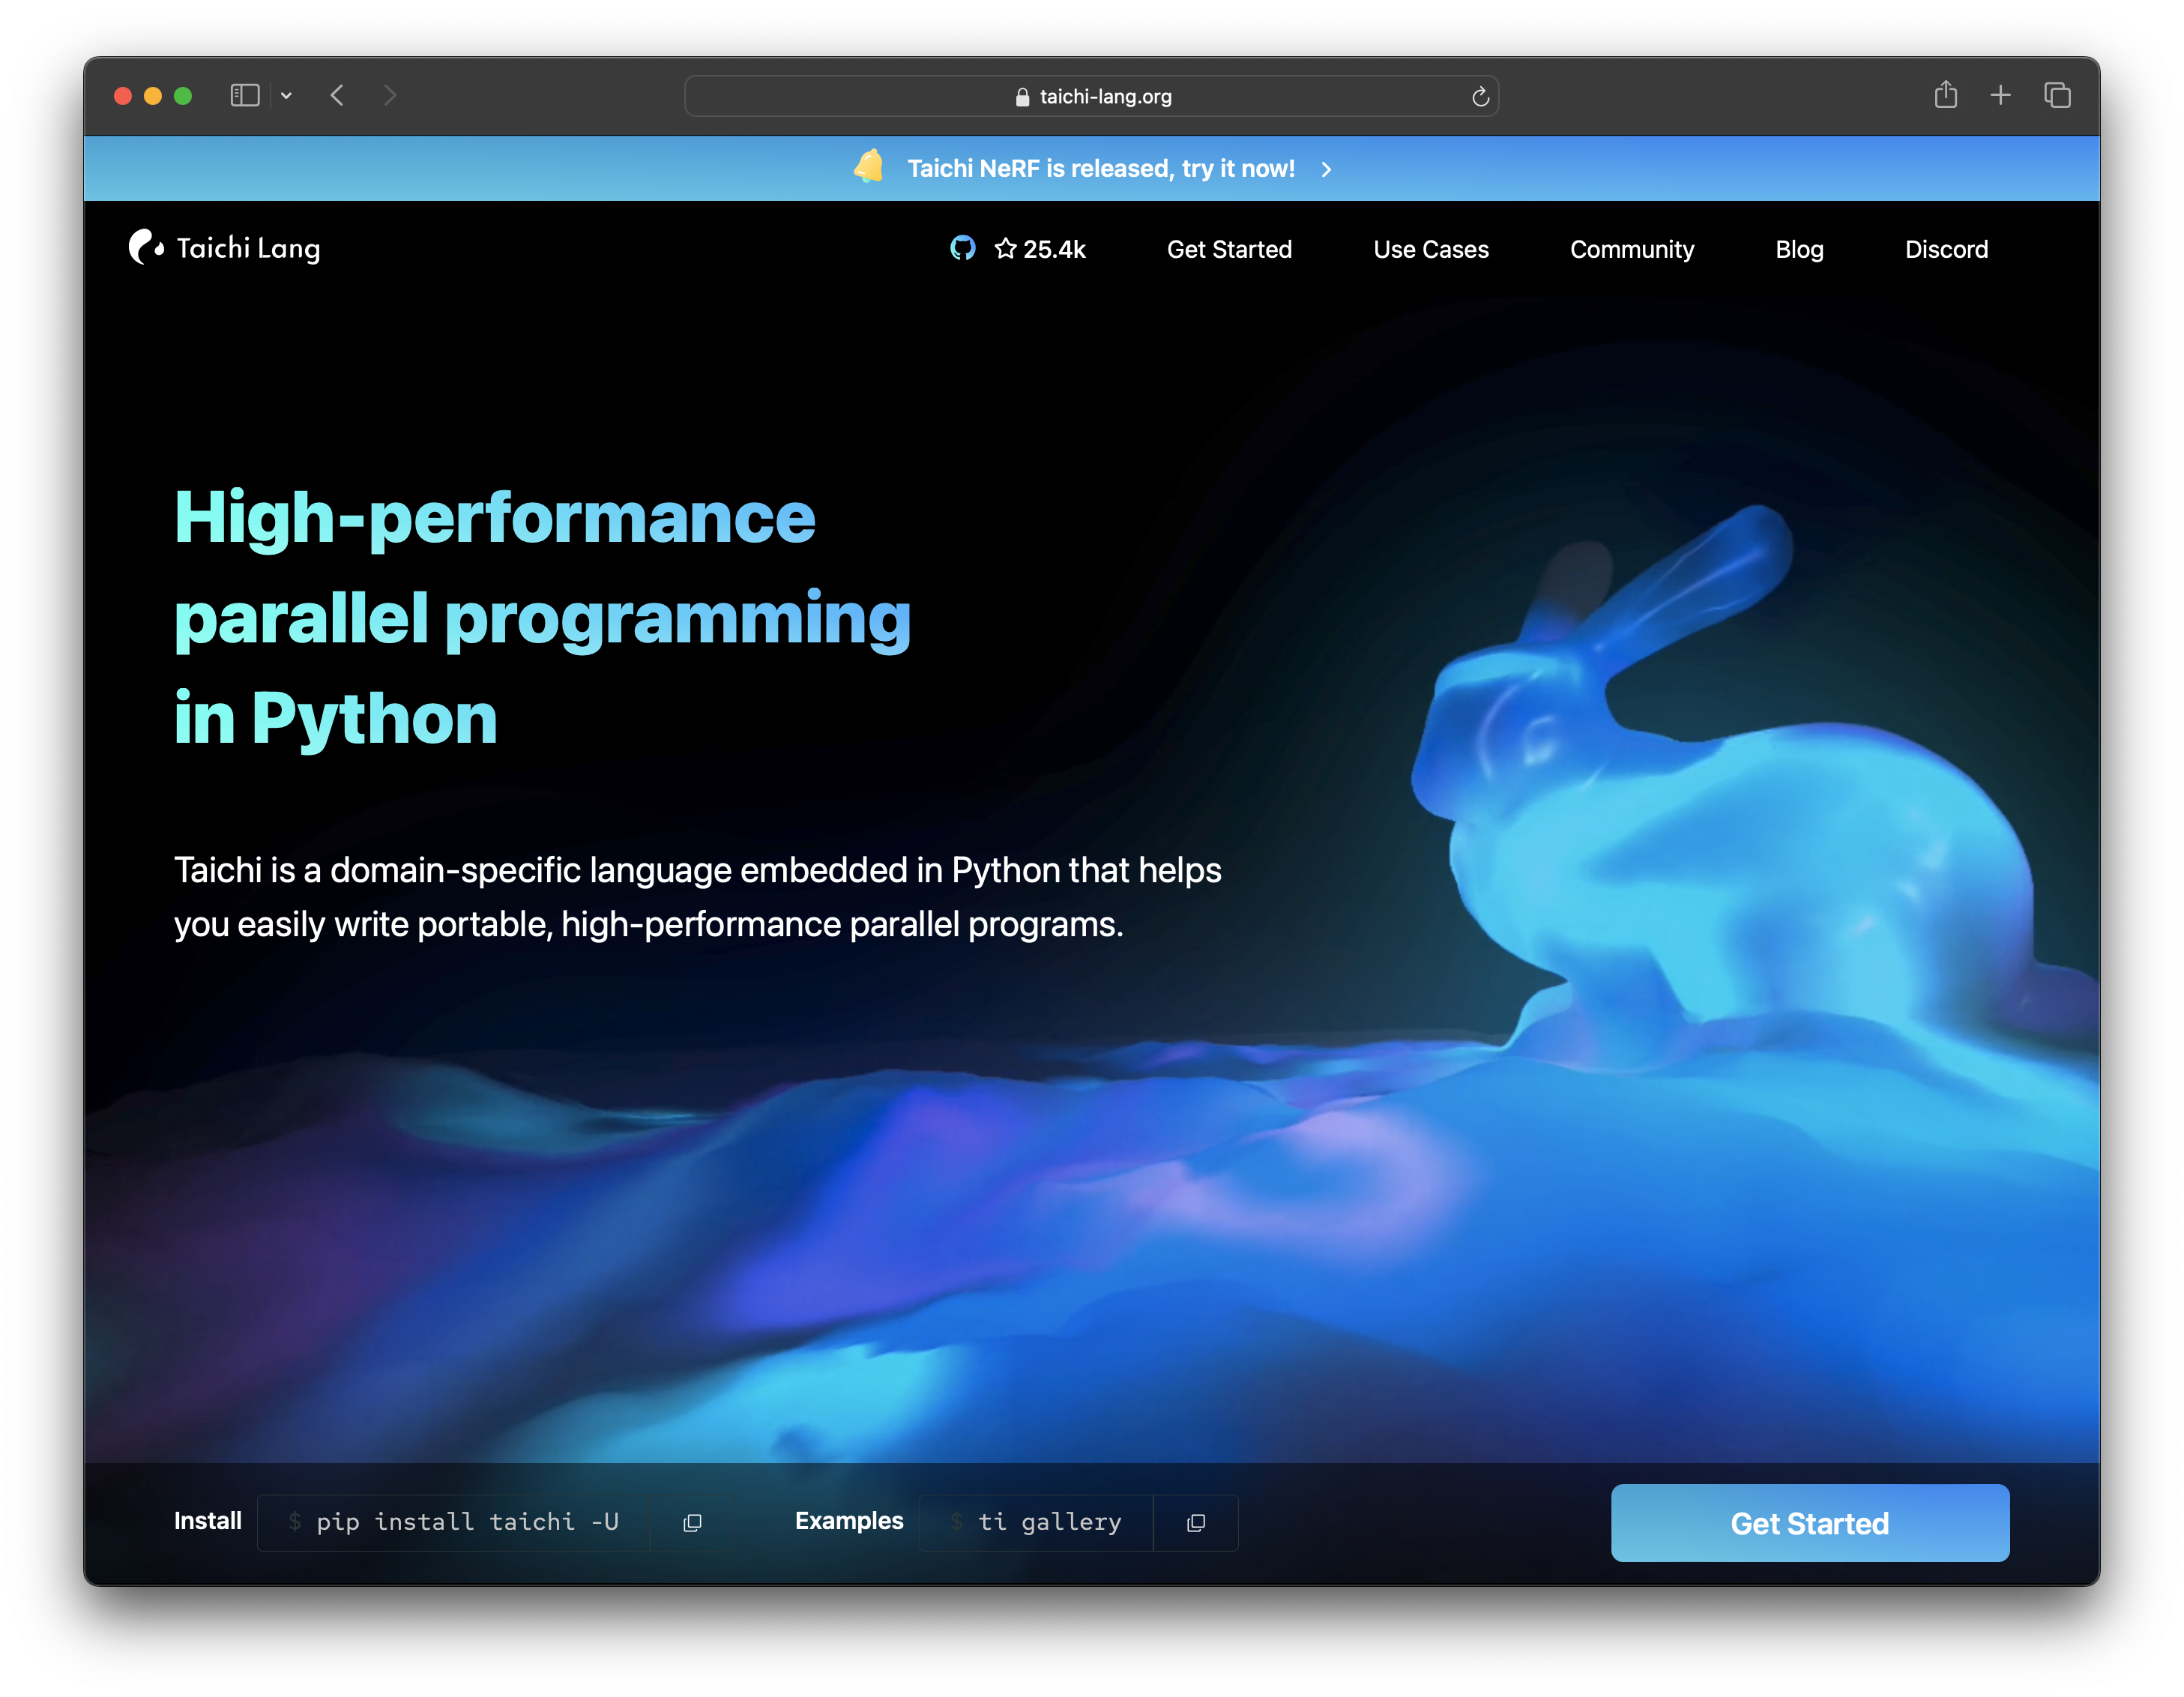
\includegraphics[width=2.5cm]{taichi_lang_org.png} 

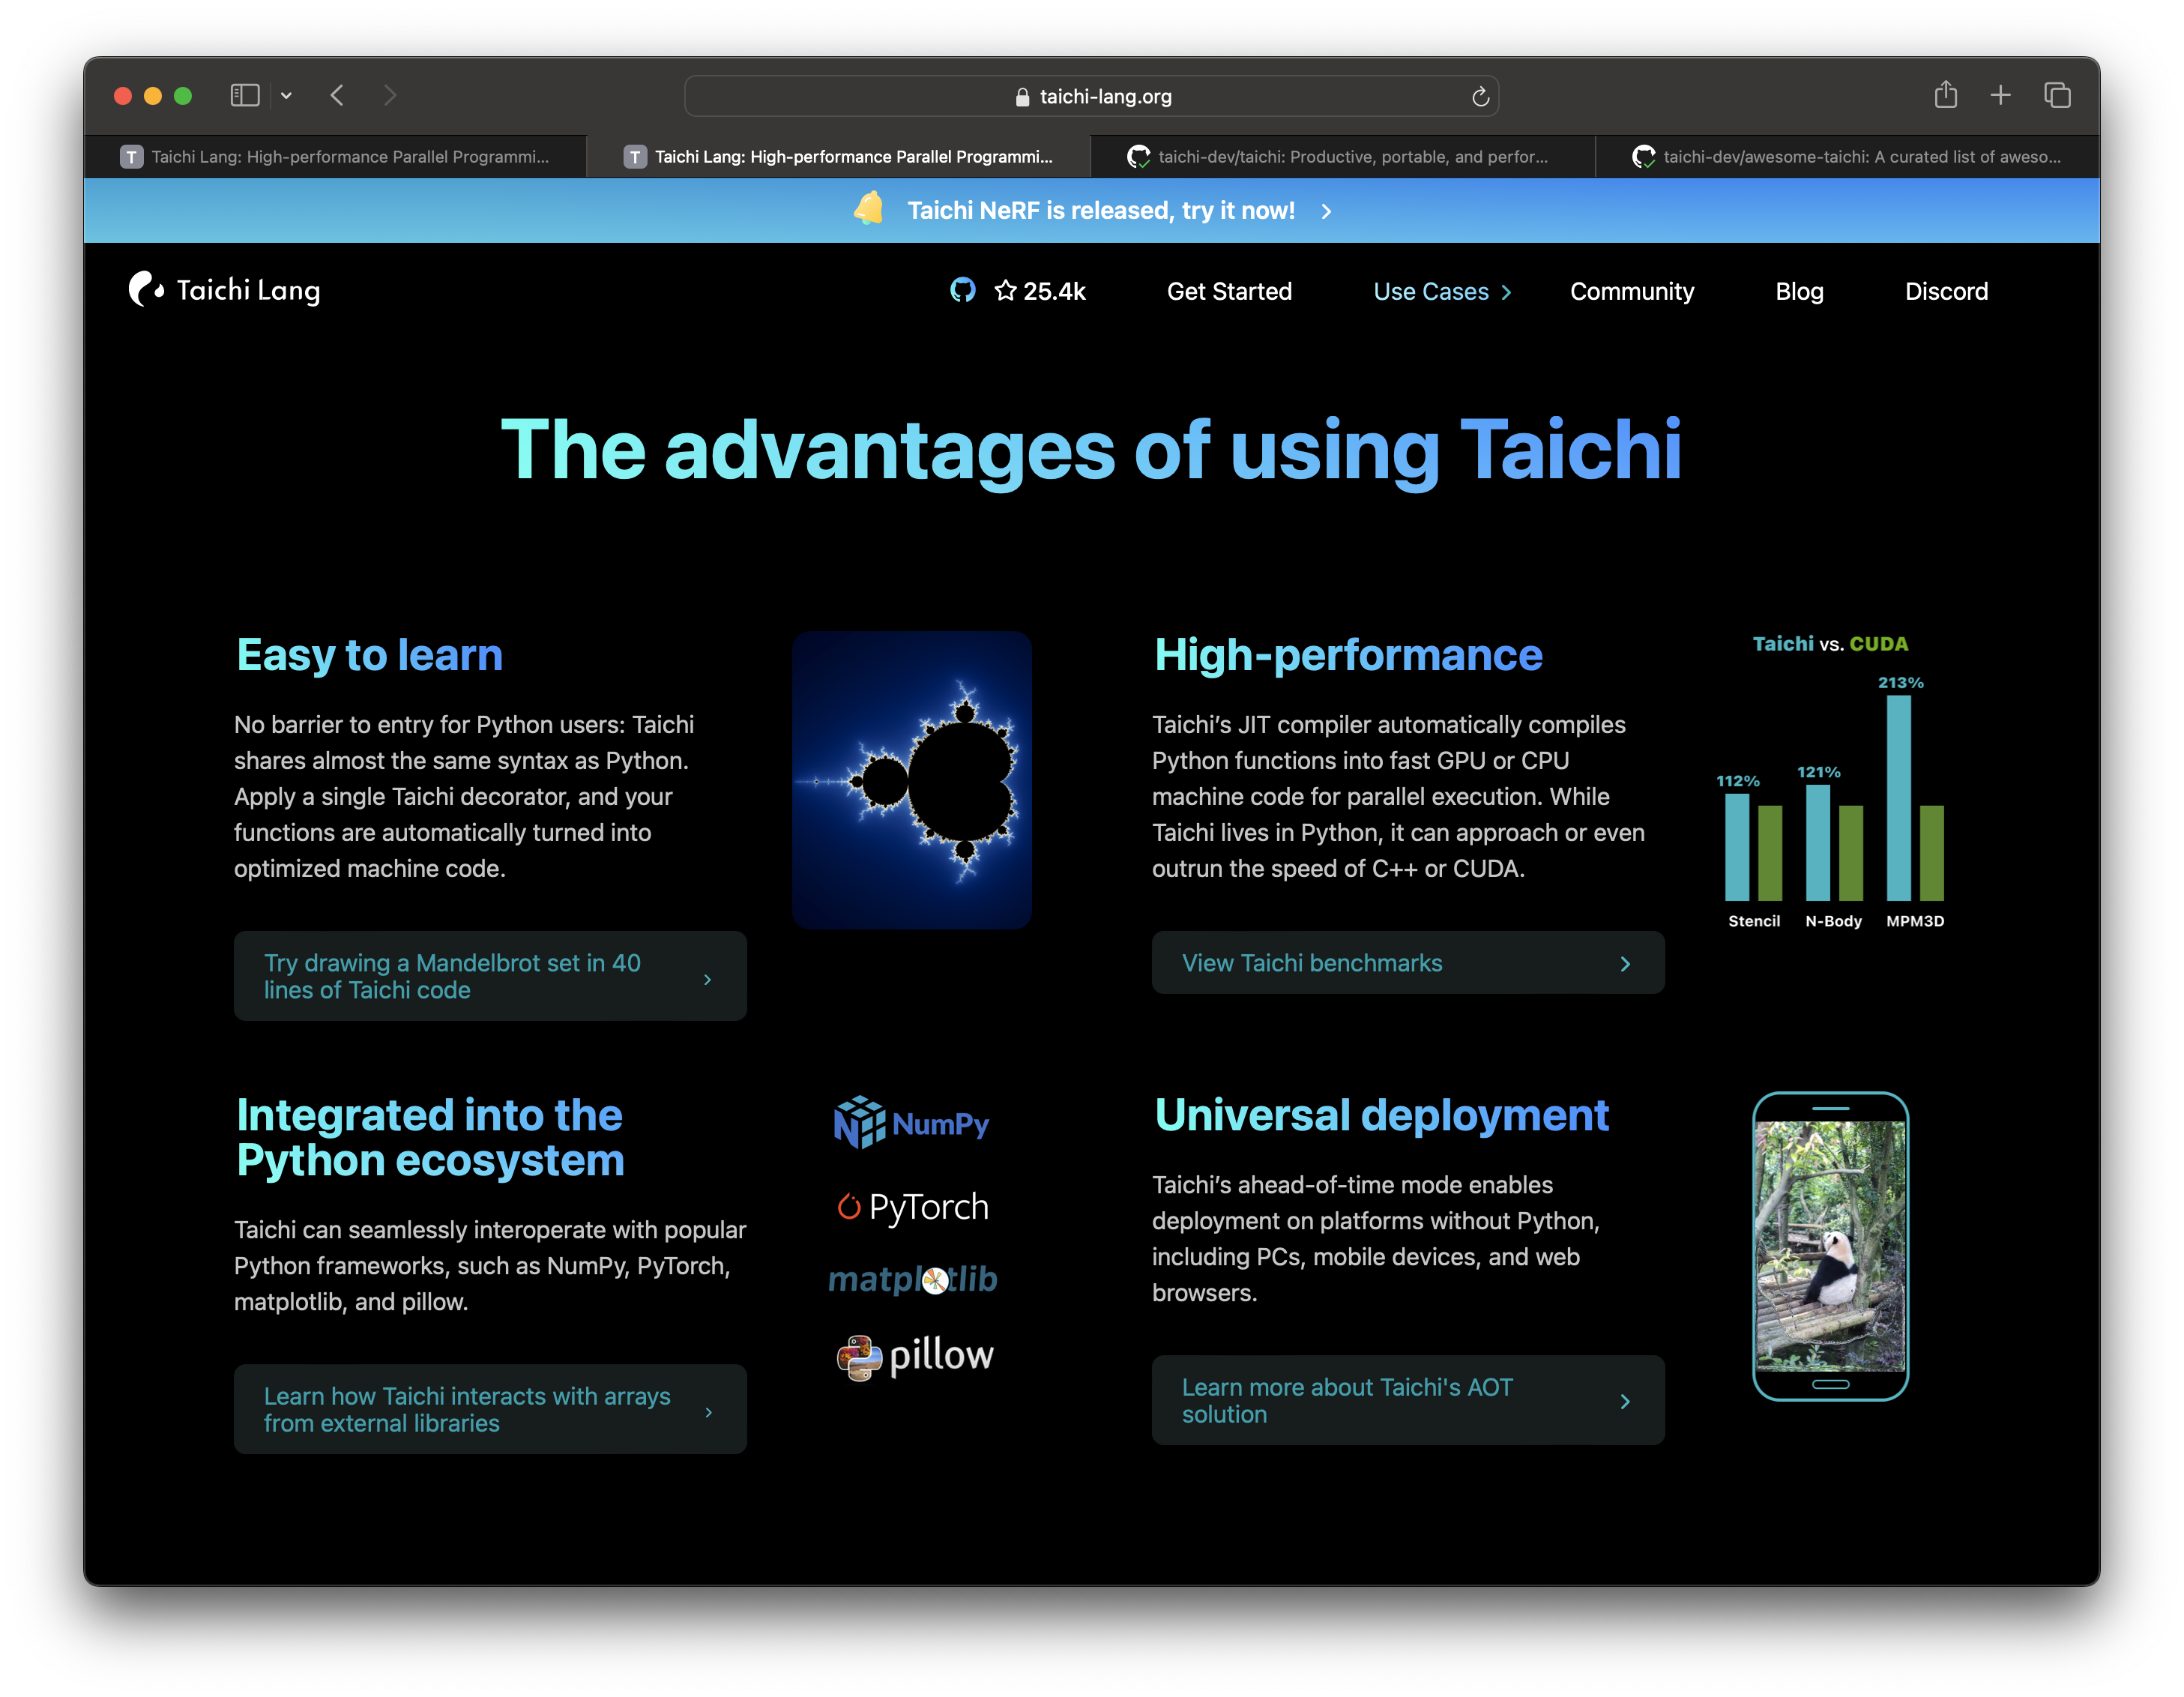
\includegraphics[width=2.5cm]{taichi_lang_org_advantages.png} 

\end{columns}
\end{frame}

\begin{frame}{Applications}
  \begin{outline}
    \1 Giga-voxel topology optimization on a single machine \cite{Liu2018}

    % Complexity of Sparse data structures
    % Freedom to explore this space
    % Add Figure 4 somewhere
  \end{outline}
\end{frame}

\begin{frame}{Life of a Taichi Kernel}
  \begin{centering}
    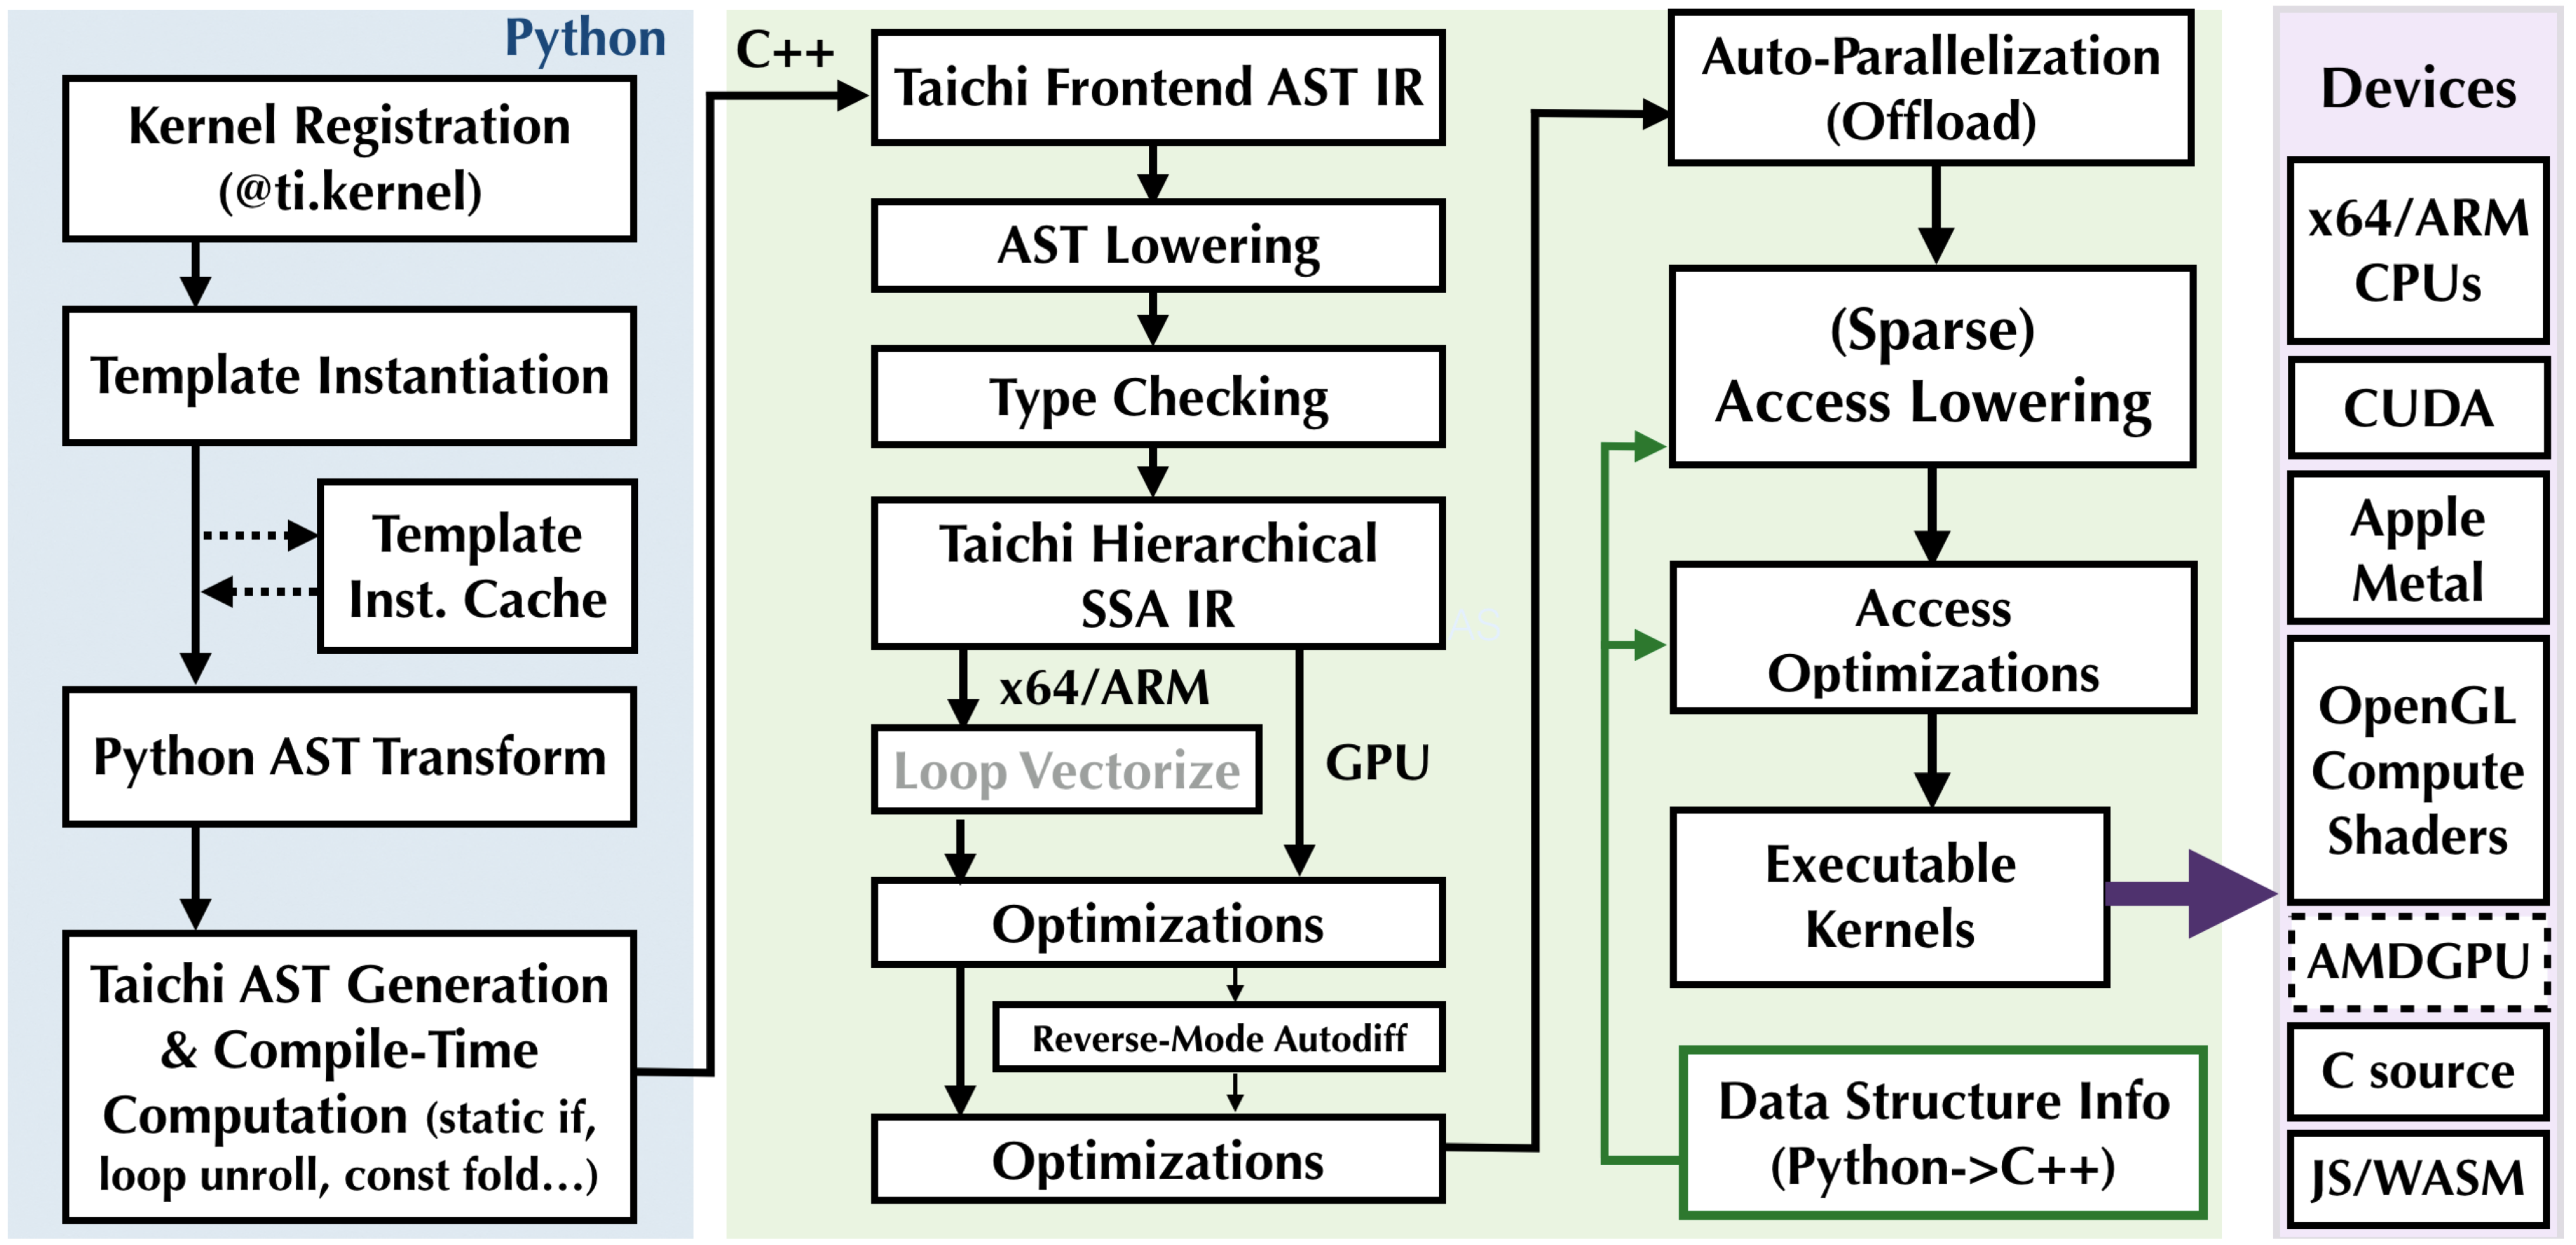
\includegraphics[width=11cm]{life_of_a_taichi_kernel.png}
  \end{centering}
\end{frame}

\begin{frame}{Why}
  \begin{outline}
    \1 Solution to a difficult area in programming 
      \2 Recreate state-of-the-art solutions 
    \1 Grown into a more general purpose tool
      \2 A fantastic edition to the python ecosystem 
      \2 Growing ecosystem (documentation, profiler, ect)
    \1 Creative Coding
      \2 Has some similarities to \href{https://processing.org}{Processing}
  \end{outline}
\end{frame}

\begin{frame}{History}
  \begin{outline}
    \1 Published ACM Transactions on Graphics 2019 \cite{Hu2019}
    \1 \href{https://yuanming.taichi.graphics/publication/2021-taichi-thesis/}{Thesis (MIT)} 
    completed in 2021
  \end{outline}
\end{frame}

\begin{frame}{Workflow}
  \begin{outline}
    \1 Write Kernels in python
    \2 Compiler 
  \end{outline}
\end{frame}

\begin{frame}{Octree}

\end{frame}

\begin{frame}{What is OpenVDB?}
  \begin{outline}
    \1 Published in ACM Trans. Graphics 2013 \cite{Museth2013}
    \1 Work was completed at Dreamworks animation
    \1 Widely used for special effects and animation
      \2 Supported by industry standard software like Houdini and Blender
  \end{outline}
\end{frame}

\begin{frame}{How does OpenVDB Work?}

\end{frame}

\begin{frame}{SPGrid}
  \begin{outline}
    \1 Published in ACM Trans. Graphics 2014 \cite{Setaluri2014}
  \end{outline}
\end{frame}

\begin{frame}[allowframebreaks]{References}
\tiny
\printbibliography
\end{frame}

\end{document}


